\chapter{Competitor Analysis}
\section{Introduction}
In this part of our diploma thesis we give you some information about our current competitors with who we are sharing our project idea.
\newline \newline
One important factor to create an outstanding product and to lead the market is to know our competitors. Like it is said “Keep your friends close, but your enemies closer”. So,  we were supposed to do some researches about similar products, which are listed on the next few pages. We try to sum up the most important facts and a short description of the products competing. 
\newline \newline
The competitor analysis showed us what we have to look at and what customers exactly need. 
\paragraph{Compared Products}
\begin{itemize}
\item Miles
\item OsmAnd
\item TOMTOM
\item Fahrtenbuch (von Stefan Meyer)
\item TOUR
\item Mileage Logbook
\item Fahrtenbuch (myLogbook)
\item MyLog GPS Fahrtenbuch Kosten
\item Carpanion
\item Fahrtenbuch Mileage Book
\item Trucker Logbook
\item Logbuch App
\item Drives Fahrtenbuch
\item Abax Triplog
\item GPS Log Book
\item GPS Log Book Live
\item Gurtam
\item Maxtech
\item Tractive
\end{itemize}
\newpage

\section{Miles}  
\begin{wrapfigure}{r}{0.5\textwidth}
  \begin{center}
    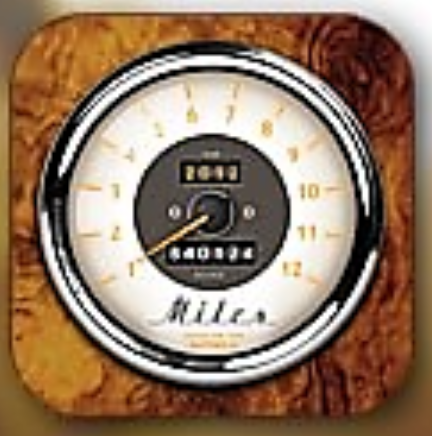
\includegraphics[width=0.48\textwidth]{bilder/miles}
  \end{center}
\end{wrapfigure}
\paragraph{Costs} \euro 39,99 once
\paragraph{Supported Platforms} The application Miles is compatible for \gls{ios} 8.
\paragraph{GPS} No \gls{gps} connection necessary.
\paragraph{Business/Private mode} You can split your private tracking from your business tracking.
\paragraph{Hardware} No Hardware. App is only used on smartphones.
\paragraph{Access Forms} App
\paragraph{Manual/Automatic Tracking} Data can only be entered manually.
\paragraph{Internet Connection} Internet connection necessary.
\paragraph{Export} It’s possible to export data to a \gls{pdf} or \gls{csv} File.
\paragraph{Other Features} No other features included.
\paragraph{References:} \cite{miles}
\newpage

\section{OsmAnd} 
\begin{wrapfigure}{r}{0.5\textwidth}
  \begin{center}
    
\includegraphics[width=0.48\textwidth]{bilder/osmand}
  \end{center}
\end{wrapfigure} 
\paragraph{Costs} \euro 6,99 once
\paragraph{Supported Platforms} For Android and \gls{ios} smartphones and tablets. Also runs on a wide array of Linux-based systems.
\paragraph{GPS} Navigation- and tracking  system in one.
\paragraph{Business/Private mode} Only private mode.
\paragraph{Hardware} No Hardware. App is only used on smartphones.
\paragraph{Access Forms} App
\paragraph{Manual/Automatic Tracking} automatic
\paragraph{Internet Connection} No Internet connection necessary.
\paragraph{Export} It’s possible to export data to a \gls{pdf} or \gls{csv} File.
\paragraph{Other Features} download offline Maps, which get used for tracking and navigation
\paragraph{References:} \cite{osmand}
\newpage

\section{TOMTOM}
\begin{wrapfigure}{r}{0.5\textwidth}
  \begin{center}
    
\includegraphics[width=0.48\textwidth]{bilder/tomtom}
  \end{center}
\end{wrapfigure}
\paragraph{Costs} \euro 69.41 once
\paragraph{Supported Platforms} For Android (2.3.3 or higher) and \gls{ios} (5.0 or higher).
\paragraph{GPS} \gls{gps} connection is necessary.
\paragraph{Business/Private mode} You can split your private tracking from your business tracking.
\paragraph{Hardware} No Hardware. App is only used on smartphones.
\paragraph{Access Forms} App
\paragraph{Manual/Automatic Tracking} No information
\paragraph{Internet Connection}No information
\paragraph{Export} It’s possible to export data to a \gls{pdf} or \gls{csv} File.
\paragraph{Other Features} No other features included.
\paragraph{References:} \cite{Electronic_Logbook_from_TOMTOM}
\newpage

\section{Fahrtenbuch (von Stefan Meyer)}
\begin{wrapfigure}{r}{0.5\textwidth}
  \begin{center}
    
\includegraphics[width=0.48\textwidth]{bilder/fahrtenbuch}
  \end{center}
\end{wrapfigure}
\paragraph{Costs} \euro 5,99 once
\paragraph{Supported Platforms} \gls{ios}
\paragraph{GPS} \gls{gps} connection is necessary.
\paragraph{Business/Private mode} You can split your private tracking from your business tracking.
\paragraph{Hardware} No Hardware. App is only used on smartphones.
\paragraph{Access Forms} App for iPhone and Apple Watch
\paragraph{Manual/Automatic Tracking} manual and automatic
\paragraph{Internet Connection} Internet connection is necessary.
\paragraph{Export} It’s possible to export data to a \gls{pdf} or \gls{csv} File.
\paragraph{Other Features} No other features included.
\paragraph{References:} \cite{Fahrtenbuch_von_Stefan_Meyer}
\newpage

\section{TOUR}
\paragraph{Source} 
\begin{wrapfigure}{r}{0.5\textwidth}
  \begin{center}
    
\includegraphics[width=0.48\textwidth]{bilder/tour}
  \end{center}
\end{wrapfigure}
\paragraph{Costs} Cost free. with features \euro 8,99 + \euro 5 to transfer the data to the computer
\paragraph{Supported Platforms} \gls{ios}
\paragraph{GPS} \gls{gps} connection is necessary.
\paragraph{Business/Private mode} You can split your private tracking from your business tracking.
\paragraph{Hardware} No Hardware. App is only used on smartphones.
\paragraph{Access Forms} App
\paragraph{Manual/Automatic Tracking} automatic
\paragraph{Internet Connection} Internet connection is necessary.
\paragraph{Export} It’s possible to export a Tax Office conform file.
\paragraph{Other Features}Trips can be combined afterwards
\paragraph{References:} \cite{TOUR}
\newpage

\section{Mileage Logbook}
\begin{wrapfigure}{r}{0.5\textwidth}
  \begin{center}
    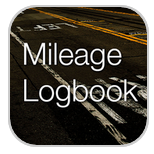
\includegraphics[width=0.48\textwidth]{bilder/mileage}
  \end{center}
\end{wrapfigure}
\paragraph{Costs} free
\paragraph{Supported Platforms} Android 
\paragraph{GPS} \gls{gps} connection is necessary.
\paragraph{Business/Private mode} You can split your private tracking from your business tracking.
\paragraph{Hardware} No Hardware. App is only used on smartphones.
\paragraph{Access Forms} App
\paragraph{Manual/Automatic Tracking} automatic
\paragraph{Internet Connection} No internet connection is necessary.
\paragraph{Export} It’s possible to export data to a \gls{html}, Excel or \gls{csv} File.
\paragraph{Other Features} No other features included.
\paragraph{References:} \cite{Mileage_Logbook}
\newpage

\section{Fahrtenbuch (myLogbook)}
\begin{wrapfigure}{r}{0.5\textwidth}
  \begin{center}
    
\includegraphics[width=0.48\textwidth]{bilder/fahrtenbuch2}
  \end{center}
\end{wrapfigure}
\paragraph{Costs} \euro 4,98 once
\paragraph{Supported Platforms} Android 
\paragraph{GPS} GPS connection is necessary.
\paragraph{Business/Private mode} Only business mode.
\paragraph{Hardware} No Hardware. App is only used on smartphones.
\paragraph{Access Forms} App
\paragraph{Manual/Automatic Tracking} automatic
\paragraph{Internet Connection} No internet connection is necessary.
\paragraph{Export} It’s possible to export data to a \gls{html}, \gls{xml}, INtex, Euro-Fahrtenbuch, Fahrtenbuch Express, WISO Fahrtenbuch or \gls{csv} File.
\paragraph{Other Features} No other features included.
\paragraph{References:} \cite{Fahrtenbuch_myLogbook}
\newpage

\section{MyLog GPS Fahrtenbuch Kosten}
\begin{wrapfigure}{r}{0.5\textwidth}
  \begin{center}
    
\includegraphics[width=0.48\textwidth]{bilder/mylog}
  \end{center}
\end{wrapfigure}
\paragraph{Costs} free
\paragraph{Supported Platforms} Android
\paragraph{GPS} \gls{gps} connection is necessary.
\paragraph{Business/Private mode} You can split your private tracking from your business tracking.
\paragraph{Hardware} No Hardware. App is only used on smartphones.
\paragraph{Access Forms} App
\paragraph{Manual/Automatic Tracking} automatic
\paragraph{Internet Connection} No internet connection is necessary.
\paragraph{Export} It’s possible to export data to a \gls{pdf} File.
\paragraph{Other Features} No other features included.
\paragraph{References:} \cite{MyLog_GPS_Fahrtenbuch_Costs}
\newpage

\section{Carpanion}
\begin{wrapfigure}{r}{0.5\textwidth}
  \begin{center}
    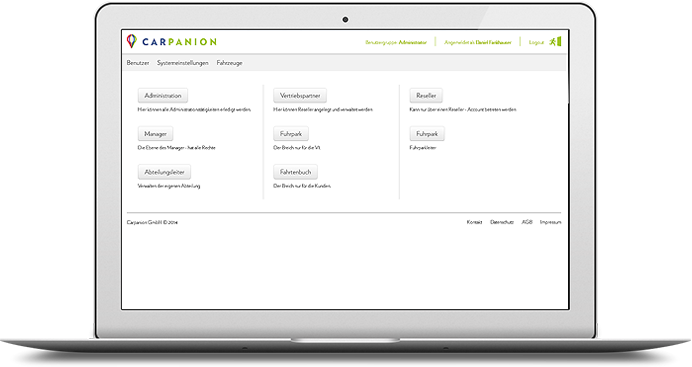
\includegraphics[width=0.48\textwidth]{bilder/Carpanion1}
  \end{center}
\end{wrapfigure}
\paragraph{Costs} free
\paragraph{Supported Platforms} Android, \gls{ios}, Windows
\paragraph{GPS} \gls{gps} connection is necessary.
\paragraph{Business/Private mode} Only private mode.
\paragraph{Hardware} No Hardware. App is only used on smartphones.
\paragraph{Access Forms}Web Form and App
\paragraph{Manual/Automatic Tracking} manual
\paragraph{Internet Connection} Internet connection necessary.
\paragraph{Export} It’s possible to export data to a \gls{pdf} or \gls{csv} File.
\paragraph{Other Features} You can take pictures of your fuel receipts and save them together with your refueling stops.
\paragraph{References:} \cite{Carpanion}
\newpage

\section{Fahrtenbuch Mileage Book}
\begin{wrapfigure}{r}{0.5\textwidth}
  \begin{center}
    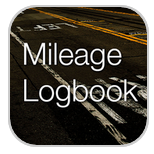
\includegraphics[width=0.48\textwidth]{bilder/mileage}
  \end{center}
\end{wrapfigure}
\paragraph{Costs} \euro 3,95 monthly (30 days testversion)
\paragraph{Supported Platforms} Android, \gls{ios}, Windows
\paragraph{GPS} \gls{gps} connection is necessary.
\paragraph{Business/Private mode} You can split your private tracking from your business tracking.
\paragraph{Hardware} No Hardware. App is only used on smartphones.
\paragraph{Access Forms} Web form, App
\paragraph{Manual/Automatic Tracking} automatic and manual
\paragraph{Internet Connection} No internet connection necessary.
\paragraph{Export} It’s possible to export data to a \gls{pdf}, \gls{xml}, Excel or \gls{csv} File.
\paragraph{Other Features} No other features included.
\paragraph{References:} \cite{Fahrtenbuch_Mileage_Book}
\newpage

\section{Trucker Logbook}
\begin{wrapfigure}{r}{0.5\textwidth}
  \begin{center}
    
\includegraphics[width=0.48\textwidth]{bilder/trucker}
  \end{center}
\end{wrapfigure}
\paragraph{Costs} free
\paragraph{Supported Platforms} Android, \gls{ios}
\paragraph{GPS} No information
\paragraph{Business/Private mode} Only business mode.
\paragraph{Hardware} No Hardware. App is only used on smartphones.
\paragraph{Access Forms}Web form, App
\paragraph{Manual/Automatic Tracking} manual
\paragraph{Internet Connection} No information
\paragraph{Export} No information
\paragraph{Other Features} No other features included.
\paragraph{References:} \cite{Trucker_Logbook}
\newpage

\section{Logbuch App}
\begin{wrapfigure}{r}{0.5\textwidth}
  \begin{center}
    
\includegraphics[width=0.48\textwidth]{bilder/logbuchapp}
  \end{center}
\end{wrapfigure}
\paragraph{Costs} \euro 5,99 once
\paragraph{Supported Platforms} \gls{ios}
\paragraph{GPS} \gls{gps} connection is necessary.
\paragraph{Business/Private mode} Only private mode.
\paragraph{Hardware} No Hardware. App is only used on smartphones.
\paragraph{Access Forms} App
\paragraph{Manual/Automatic Tracking} No information
\paragraph{Internet Connection} No information
\paragraph{Export} It’s possible to export data to a \gls{pdf} File, Excel or \gls{csv} File.
\paragraph{Other Features} Weather
\paragraph{References:} \cite{Logbuch_App}
\newpage

\section{Drives Fahrtenbuch}
\begin{wrapfigure}{r}{0.5\textwidth}
  \begin{center}
    
\includegraphics[width=0.48\textwidth]{bilder/drives}
  \end{center}
\end{wrapfigure}
\paragraph{Costs} Cost free, but there's also a chargeable version where private routes get tracked automatically and you can register more than one vehicle.
\paragraph{Supported Platforms} \gls{ios}
\paragraph{GPS} No information
\paragraph{Business/Private mode} You can split your private tracking from your business tracking.
\paragraph{Hardware} No Hardware. App is only used on smartphones.
\paragraph{Access Forms} App
\paragraph{Manual/Automatic Tracking} The manual tracking version is cost free, but at the chargeable version the automatic tracking is possible and you can split your private and business tracking.
\paragraph{Internet Connection} No information
\paragraph{Export} It’s possible to export data to a \gls{pdf} or \gls{csv} File.
\paragraph{Other Features} 
\begin{itemize}
\item You can use \gls{db} entries as pattern for future tracks
\item Statistics
\item Backups
\item In the chargeable version of the app, you can register more than one vehicle
\end{itemize}
\paragraph{References:} \cite{Drives_Fahrtenbuch}
\newpage

\section{Abax Triplog}
\begin{wrapfigure}{r}{0.5\textwidth}
  \begin{center}
    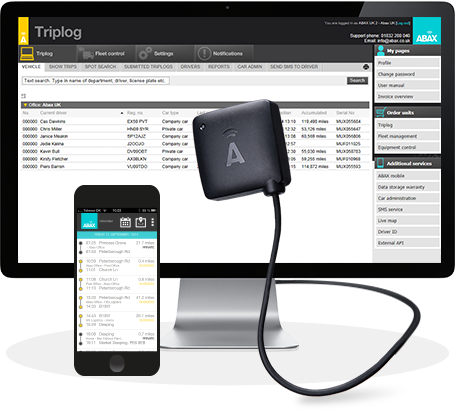
\includegraphics[width=0.48\textwidth]{bilder/abax}
  \end{center}
\end{wrapfigure}
\paragraph{Costs} \euro 35,29 monthly \& \euro 249,00 Hardware
\paragraph{Supported Platforms} \gls{ios}
\paragraph{GPS} \gls{gps} connection is necessary.
\paragraph{Business/Private mode} You can split your private tracking from your business tracking.
\paragraph{Hardware}The hardware is very robust and waterproof.
\paragraph{Access Forms}Web form, App
\paragraph{Manual/Automatic Tracking}automatic
\paragraph{Internet Connection}Internet connection necessary.
\paragraph{Export}No information
\paragraph{Other Features} 
\begin{itemize}
\item Contract period of 3 years
\item Lifetime Warranty
\end{itemize}
\paragraph{References:} \cite{Abax_Triplog}
\newpage

\section{GPS Log Book}
\begin{wrapfigure}{r}{0.5\textwidth}
  \begin{center}
    
\includegraphics[width=0.48\textwidth]{bilder/GPSlogbook}
  \end{center}
\end{wrapfigure}
\paragraph{Costs} \euro 117,11 + \euro 26,33 per year
\paragraph{Supported Platforms} Web interface
\paragraph{GPS} \gls{gps} connection is necessary.
\paragraph{Business/Private mode} Only private mode.
\begin{wrapfigure}{r}{0.5\textwidth}
  \begin{center}
    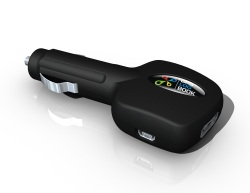
\includegraphics[width=0.48\textwidth]{bilder/GPSlogbook2}
  \end{center}
\end{wrapfigure}
\paragraph{Hardware}The product consists of a plug in for the car.
\paragraph{Access Forms} Web form
\paragraph{Manual/Automatic Tracking}automatic, manual
\paragraph{Internet Connection}Internet connection is necessary, but data doesn't get transmitted to the \gls{db}.
\paragraph{Export}It's possible to export data to a \gls{pdf} or \gls{csv} File.
\paragraph{Other Features}
\begin{itemize}
\item 5 years data retention 
\item Google Maps integrated
\item 4\gls{mb} log data on the device
\end{itemize}
The GPS Log Book device plugs into a cigarette lighter socket. You have to copy the data manually from the GPS Log Book on you PC.
\paragraph{References:} \cite{GPS_Log_Book}
\newpage

\section{GPS Log Book Live}
\begin{wrapfigure}{r}{0.5\textwidth}
  \begin{center}
    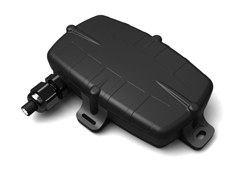
\includegraphics[width=0.48\textwidth]{bilder/GPSlogbooklive!}
  \end{center}
\end{wrapfigure}
\paragraph{Costs}\euro 416,69 + \euro 18,16 monthly + Installation \euro 89,87 
\paragraph{Supported Platforms} Web interface
\paragraph{GPS} \gls{gps} connection is necessary.
\paragraph{Business/Private mode}You can split your private tracking from your business tracking.
\paragraph{Hardware}The hardware is very robust and waterproof.
\paragraph{Access Forms}Web form
\paragraph{Manual/Automatic Tracking}automatic + manual
\paragraph{Internet Connection}Internet connection necessary.
Data gets automatically  transmitted to the \gls{db}.
\paragraph{Export}It’s possible to export data to a \gls{pdf} or \gls{csv} File.
\paragraph{Other Features}
\begin{itemize}
\item 5 years data retention  
\item Google Maps integrated
\item Live
\end{itemize}
\paragraph{References:} \cite{GPS_Log_Book_LIVE}
\newpage

\section{Gurtam}
\begin{wrapfigure}{r}{0.5\textwidth}
  \begin{center}
    
\includegraphics[width=0.48\textwidth]{bilder/gurtam}
  \end{center}
\end{wrapfigure}
\paragraph{Costs} No information 
\paragraph{Supported Platforms} Every platform which supports  Google Chrome 20+, Firefox 15+, Safari 5+, IE 9+, Opera 10+
\paragraph{GPS} \gls{gps} connection is not necessary.
\paragraph{Business/Private mode} You can split your private tracking from your business tracking.
\paragraph{Hardware}No Hardware. App is only used on smartphones.
\paragraph{Access Forms}Web form
\paragraph{Manual/Automatic Tracking}manual
\paragraph{Internet Connection}No internet connection is necessary.
\paragraph{Export}It’s possible to export data to different Files.
\paragraph{Other Features}
\begin{itemize}
\item specifying the beginning and the end of the trip;
choosing type (business/personal trip);
\item specifying initial and final position, duration, mileage data, etc.;
\item manual adding columns containing user notes;
\item logging all the changes;
\item printing or exporting to file;
\item setting Costs per kilometer or per litre (in case of personal trip it helps to calculate the total Costs).
\end{itemize}
\paragraph{References:} \cite{Gurtam_Wialon_Driving_Logbook}
\newpage

\section{Maxtech}
\begin{wrapfigure}{r}{0.5\textwidth}
  \begin{center}
    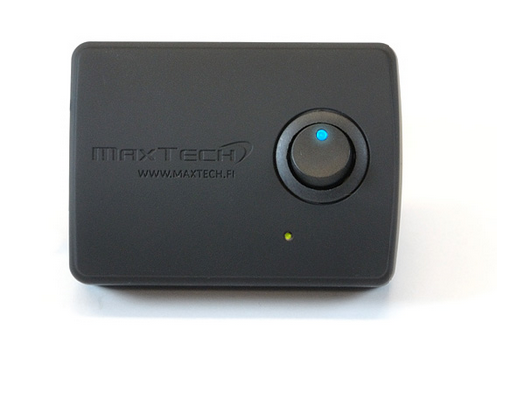
\includegraphics[width=0.48\textwidth]{bilder/logbook}
  \end{center}
\end{wrapfigure}
\paragraph{Costs} \euro 189 once
service fee (including the service, SIM card and subscription) is roughly \euro 20 per month (prices excl. VAT)
\paragraph{Supported Platforms} No information given
\paragraph{GPS} \gls{gps} connection is necessary.
\paragraph{Business/Private mode}You can split your private tracking from your business tracking.
\paragraph{Hardware}Hardware is included (picture on the right)
\paragraph{Access Forms}Web form
\paragraph{Manual/Automatic Tracking}automatic and manual
\paragraph{Internet Connection}Yes, data gets transmitted to a server
\paragraph{Export}It is  possible to export data to a \gls{pdf} or \gls{csv} File.
\paragraph{Other Features}
\begin{itemize}
\item An automatic logbook remembers to collect all the drive data so you will no longer forget any travels.
\item data is available anywhere and anytime
\item track your car when the driver is someone else and it also helps if your car is stolen – a tracking device will send the location of your car when it moves.
\item if no internet is available, the drive data gets stored on an internal buffer memory, which can save up to 2000 km
\end{itemize}
Vehicle tracking devices can be installed in three different ways:
\begin{itemize}
\item Cigarette lighter plug
\item OBD connector
\item Fixed mounting to car battery (10V-30V)
\end{itemize}
\paragraph{References:} \cite{Maxtech}
\newpage

\section{Tractive}
\begin{wrapfigure}{r}{0.5\textwidth}
  \begin{center}
    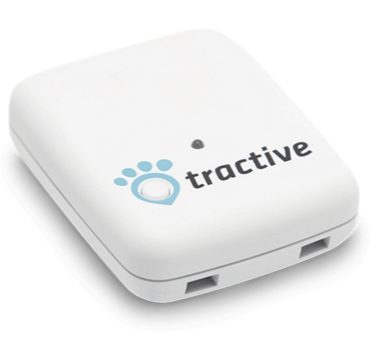
\includegraphics[width=0.48\textwidth]{bilder/tractive}
  \end{center}
\end{wrapfigure}
\paragraph{Costs}\euro 79.99 once + \euro 4.99 or \euro 7.49 (Premium) per month 
\paragraph{Supported Platforms}Android and \gls{ios} 
\paragraph{GPS} \gls{gps} connection is necessary.
\paragraph{Business/Private mode} -
\paragraph{Hardware}Hardware is included (picture on the right)
\paragraph{Access Forms}App
\paragraph{Manual/Automatic Tracking}automatic
\paragraph{Internet Connection}Yes, data gets transmitted on the smartphone of the user.
\paragraph{Export}-
\paragraph{Other Features}
\begin{itemize}
\item Sensors for:
\begin{itemize}
\item Movement
\item Speed-Up
\item Temperature
\item Brightness
\end{itemize}
\item Waterproof
\item Alarm, if the pet leaves a certain area
\end{itemize}
\paragraph{References:}\cite{Tractive}
\newpage

\section{Summary}
Most of the products only run on very few or only on one platform. Also, there are different versions of software (pay/free) which divide the user experience in either good or bad way. Therefore, our idea is a single software with an extra hardware, web form and an app, which runs on IOS, Android and also on Windows phones. This main functionalities should distinguish us from the rest of the market. 
\newline\newline
In the analysis above you can see some of the most important competitor products. In our opinion, the largest competitors are Mileage Book and Fahrtenbuch (von Stefan Meyer). These products have many features and a very low or rather no price. However, their product only includes an App.
On the hardware side, GPS Log Book Live and the company maxtech with their product Automatic Driver’s Logbook are our biggest competitors, but although their product is highly innovative, there is no App in the product included. Secondly, the product of the company Tractive, which should help not to lose your pet, but it also shows the activeness of the pet during a certain day time and temperature.
\newline\newline
In conclusion, there is actually no product which has both a hardware and an app. There are only two products which includes both. On the one hand it is Tractive, which is only for animals though. On the other hand, it is Abax Triplog. However, their software only runs on IOS. So, the hardware and app in one will distinguish ourselves from the others.
\newline\newline

\begin{tabular}{p{4cm}p{5cm}p{3cm}p{2cm}}
\toprule

  \textbf{Name of Product} & \textbf{Costs} & \textbf{Supported Plattform} & \textbf{includes Hardware} \\
\midrule
  Miles                      & \euro 39,99                                                                                                 & IOS 8                 & No  \\ 
OsmAnd                     & \euro 6,99                                                                                                  & IOS, Tablets, Linux   & No  \\ 
TOMTOM                     & \euro 69,41                                                                                                 & Android and IOS       & No  \\ 
Fahrtenbuch (Stefan Meyer) & \euro 5,99                                                                                                  & IOS                   & No  \\ 
TOUR                       & free                                                                                                        & IOS                   & No  \\ 
Mileage Logbook            & free                                                                                                        & Android               & No  \\ 
Fahrtenbuch (myLogbook)    & \euro 4,98                                                                                                  & Android               & No  \\ 
MyLog GPS Fahrtenbuch      & free                                                                                                        & Android               & No  \\ 
Carpanion                  & free                                                                                                        & Android, IOS, Windows & No  \\ 
Fahrtenbuch Mileage Book   & \euro 3,95 per Month                                                                                        & Android, IOS, Windows & No  \\ 
Trucker Logbook            & free                                                                                                        & Android, IOS          & No  \\ 
Logbuch App                & \euro 5,99                                                                                                  & IOS                   & No  \\ 
Drivers Fahrtenbuch        & free                                                                                                        & IOS                   & No  \\ 
Abax Triplog               & \euro 35,29 per Month + \euro 249 Hardware                                                                  & IOS                   & Yes \\ 
GPS Log Book               & \euro 117,11 + \euro 26,33 per Year                                                                         & Web interface         & Yes \\ 
GPS Log Book Live          & \euro 416,69 + \euro 18,16 per Month + \euro 89,87\\   Installation & Web interface         & Yes \\
Gurtam                     & No information                                                                                              & Web interface         & No  \\ 
Maxtech                    & \euro 189                                                                                                   & No information        & Yes \\ 
Tractive                   & \euro 79,99 once + \euro 4,99 or \euro 7,99 (Premium)per Month                                              & Andoid, IOS           & Yes \\ 
\bottomrule
\end{tabular}

